\documentclass[12pt]{article}
\usepackage{graphicx}
\usepackage{caption}
\usepackage{subcaption}
\usepackage{tikz}
\usepackage{venndiagram}
\usepackage{venndiagram}
\usepackage{tcolorbox}
\usepackage{listings}
\usepackage{enumitem}
\usepackage{amsmath}
\usepackage{amssymb}
\usepackage{colortbl}
\usepackage{xcolor}
\usepackage[margin=1cm, top=1.5cm, bottom=1.5cm]{geometry}

\tcbuselibrary{breakable}

\title{\textbf{Gráficas y Juegos: Tarea 02}}
\author{Martínez Méndez Ángel Antonio\\Pinzón Chan José Carlos\\Rendón Ávila Jesús Mateo}
\date{\today}

\begin{document}

\maketitle
\begin{center}
\vspace{3cm}
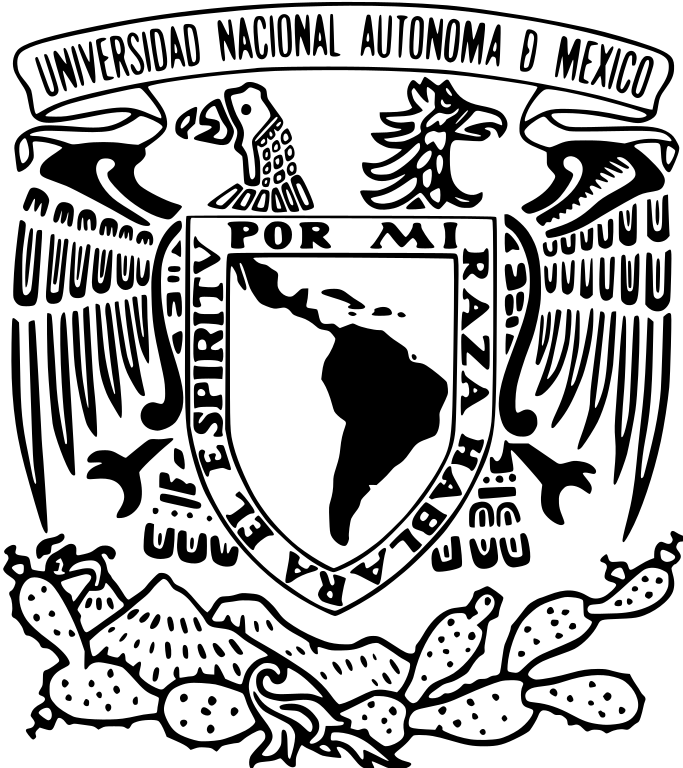
\includegraphics[width=0.195\textwidth]{Escudo.png}
\hspace{0.5cm}
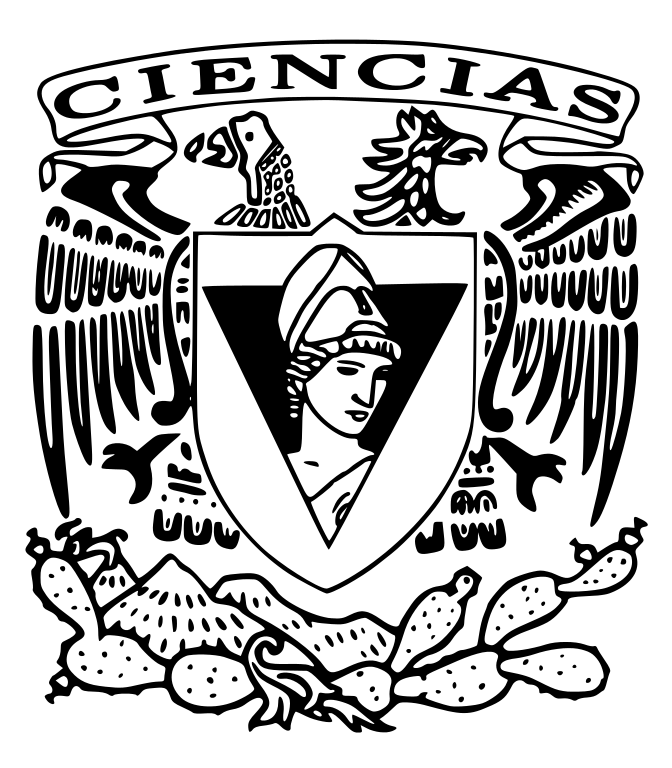
\includegraphics[width=0.2\textwidth]{logo_ciencias.png}
\end{center}
\begin{center}
    \vspace{1cm}
    Universidad Nacional Autónoma de México\\
    Facultad de Ciencias\\
    Profesor: César Hernández Cruz\\
\end{center}

\newpage

%
% Ejercicio 1
%
\textbf{1.} Sea $G$ una gáfica, y recuerde que $c_G$ denota al número de componentes conexas de $G$.
Demuestre que si $e \in E$, entonces $c_G \leq c_{G - e} \leq c_G + 1$.\\

\begin{tcolorbox}[title=\textbf{Hipotesis}, colback=red!15!white, colframe=black!, breakable]
	$G$ es una  gráfica cuyo número de componentes conexas se denota $c_G$ y $e = uv$ es una arista tal que $e \in E_G$
\end{tcolorbox}

\begin{tcolorbox}[title=\textbf{Definiciones}, colback=blue!15!white, colframe=black!, breakable]
    $Def$. A las subgráficas de una gráfica G, máximas por contención con la propiedad de ser conexas, se les llama \textbf{componentes conexas}.
\end{tcolorbox}

Por hipótesis el número de componentes conexas de $G$ es $c_G$. Sabemos que $e \in E_G$ por lo cual $e$ forma parte de alguna componente conexa en G. Como se trata de componentes conexas , entre cualesquiera vértices que pertenezcan a la misma componente conexa que $e$,  existe un $camino$. A partir de este punto se pueden distinguir dos casos generales:\\

Sean $x,y$ dos vértices en la misma componente conexa que $e$.
\begin{enumerate}
 	\item [1)] Existe un $xy-camino$, llamémoslo  $W$, tal que $e$ no forma parte de $W$:\\
	En este caso, como $e$ no forma parte de W entonces al eliminar dicha arista el $xy-camino$ sigue existiendo.
	\item [2)]Existe un $xy-camino$, llamémoslo  $P$, tal que $e$ forma parte de $P$. En este segundo caso es donde divergen dos posibilidades muy 				importantes:
	\begin{enumerate}	
		\item Si entre los vértices $u$ y $v$ existe un $uv-camino$ distinto de \{$u$,$e$,$v$\}, que denotaremos como R, al eliminar la arista $e$ de G, el 	camino P ya no coneca a $x$ con $y$, sin embargo, prevalece un $xy-camino$ descrito del siguiente modo: $xPuRvPy$. En 	consiguiente podemos decir que la grafica sigue siendo conexa y que por lo tanto $c_{G-e}$ = $c_G$.
		
		\item Si entre los vértices $u$ y $v$ el único camino existente es \{$u$,$e$,$v$\}, al eliminar $e$ de G, el camino P deja de 		existir y sucede que $u$ no puede alcanzar a $v$. Como resultado $x$ no puede alcanzar a $y$, oséase, no existe un $xy-camino$; la componente conexa se ha separado.Por el incisio 1), sabemos que todos los caminos en los que $e$ no forma parte se conservan, por lo tanto, en ambas particiones la grafica sigue 	siendo conexa. Asi podemos concluir que $c_{G-e}$ = $c_G$ + 1.
	\end{enumerate}	
\end{enumerate}

A manera de resumen, puede suceder que $c_G$ = $c_{G-e}$, o bien, $c_{G-e}$ = $c_G$ + 1, en otras palabras: $c_G \leq c_{G - e} \leq c_G + 1$.\\

\textit{Nota: Eliminar a la arista \underline{e} no afecta a las componentes conexas a las que \underline{e} no pertenece, es por ello que ignoramos al resto de componentes y nos centramos en la componente de \underline{e}.}


\vspace{1cm}

%
% Ejercicio 2
%
\textbf{2.} Una gráfica es \textit{escindible} completa si su conjunto de vértices admite una partición $(S, K)$
de tal forma que S es un conjunto independiente, $K$ es un clan, y cada vértice en $S$ es
adyacente a cada vértice en $K$. Demuestre que una gráfica es escindible completa si y
sólo si no contiene a $C_4$ ni a $\overline{P_3}$ como subgráfica inducida. (Sugerencia: Un ejercicio de
la tarea anterior puede resultar de utilidad.)
\vspace{1cm}

%
% Ejercicio 3
%
\textbf{3}.

\begin{enumerate}[label=\alph*)]

    \item Demuestre que si $\mid E \mid > n - 1$, entonces $G$ es conexa.
    \begin{tcolorbox}[title=\textbf{Hipotesis}, colback=red!15!white, colframe=black!]

    \end{tcolorbox}
    \begin{tcolorbox}[title=\textbf{Definiciones}, colback=blue!15!white, colframe=black!]
    
    \end{tcolorbox}

    \item Para cada $n > 3$ encuentre una gráfica inconexa de orden $n$ con $|E| = n - 1$.
    \begin{tcolorbox}[title=\textbf{Hipotesis}, colback=red!15!white, colframe=black!]

    \end{tcolorbox}
    \begin{tcolorbox}[title=\textbf{Definiciones}, colback=blue!15!white, colframe=black!]
    
    \end{tcolorbox}
\end{enumerate}

\vspace{1cm}
%
% Ejercicio 4
%
\textbf{4.}
\begin{enumerate}[label=\alph*)]

    \item Demuestre que si $\delta >  \left( \left\lfloor \frac{|V|}{2} \right\rfloor - 1 \right)$, entonces $G$ es conexa.
    \begin{tcolorbox}[title=\textbf{Hipotesis}, colback=red!15!white, colframe=black!]
        El grado minimo $\delta$ de $G$ es mayor a $\left( \left\lfloor \frac{|V|}{2} \right\rfloor - 1 \right)$.
    \end{tcolorbox}

        Sea $G$ una gráfica cuyo grado minimo es $\delta > \left( \left\lfloor \frac{|V|}{2} \right\rfloor - 1 \right)$, entonces
        podemos decir quev $\delta \geq  \left\lfloor \frac{|V|}{2} \right\rfloor - 1 + 1$, es decir:

        \begin{center}
        $\delta \geq  \left\lfloor \frac{|V|}{2} \right\rfloor$
        \end{center}

        Si $S$ es un subconjunto de $ V(G)$ que satisface $|S| = |V| - 2$ y $u$, $v$ dos vértices
        que pertenecen a $V(G)$ y no pertenecen a $S$.\\

        Como sabemos que $u, v \notin S$. Si es que $u$ es adyacente 
        a $\frac{|S|}{2}$ elementos $s \in S$ y $v$ es adyacente a $\frac{|S|}{2}$ elementos $s' \in S$, es decir,
        $u$ es adyacente a $\frac{|V| - 2}{2}$ elementos $s \in S$ y $v$ es adyacente a
        $\frac{|V| - 2}{2}$ elementos $s' \in S$. Con lo anterior podemos decir que $u$ es adyacente a los elementos del 
        subconjunto de $S$ $\{s_0, s_1, s_2, \dots, s_n\}$, mientras que $v$ es adyacente a los elementosdel subconjunto de $S$
        $\{s'_0, s'_1, s'_2, \dots, s'_n\}$\\

        Como por hipotesis sabemos que $d(u), d(v) \geq \left\lfloor \frac{|V|}{2} \right\rfloor$, entonces cuando
        $|V|$ es impar debe haber un $s^{\ast}$ en $S$ tal que $s_n = s^{\ast} = s'_n$.
        Mientras que cuando $|V|$ es par, existe otro $s^{\ast \ast}$ que cumple $s_i = s^{\ast \ast} = s'_i$ a los cuales $u$ y $v$ son adyacentes.
        Por lo que podemos grantizar una $uv$- trayectoria $P$:
        
        \begin{center}
            $P = (u, s_n = s^{\ast} = s'_n, v)$ cuando $|V|$ es par e impar y\\

            $P' = (u, s_n = s^{\ast \ast} = s'_n, v)$, cuando $|V|$ es par
        \end{center}

        para cada $u, v \in V(G)$. Por lo tanto $G$ es conexa.\\
        \begin{figure}[h!]

        \centering
        \begin{minipage}{0.2\textwidth}
            \centering
        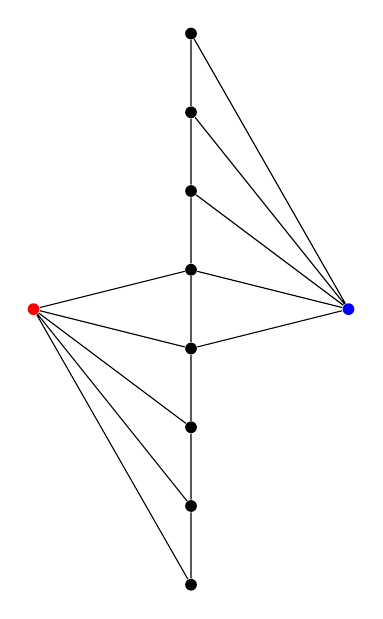
\begin{tikzpicture}[scale=1]
            \node (a) at (2,0) [circle,fill,inner sep=1.5pt] {};
            \node (b) at (2,1) [circle,fill,inner sep=1.5pt] {};
            \node (c) at (2,2) [circle,fill,inner sep=1.5pt] {};
            \node (d) at (2,3) [circle,fill,inner sep=1.5pt] {};
            \node (e) at (2,4) [circle,fill,inner sep=1.5pt] {};
            \node (f) at (2,5) [circle,fill,inner sep=1.5pt] {};
            \node (g) at (2,6) [circle,fill,inner sep=1.5pt] {};
            \node (h) at (2,7) [circle,fill,inner sep=1.5pt] {};

            \node (u) at (0,3.5) [circle,fill,inner sep=1.5pt, color=red] {};
            \node (v) at (4,3.5) [circle,fill,inner sep=1.5pt, color=blue] {};
            \draw (u) -- (a) (u) -- (b) (u) -- (c) (u) -- (d) (u) -- (e) (v) -- (e) (v) -- (f) (v) -- (g) (v) -- (h) (v) -- (d)
            (a) -- (b) (b) -- (c) (c) -- (d) (d) -- (e) (e) -- (f) (f) -- (g) (g) -- (h);
        \end{tikzpicture}
            \caption{\scriptsize Representación de $G$ cuando $|V|$ es par, suponiendo que en la columna central (negra) son adaycentes cualesqueira 2 vértices.}

       \end{minipage}
        \hspace{0.1\textwidth}
        \begin{minipage}{0.2\textwidth}
            \centering
        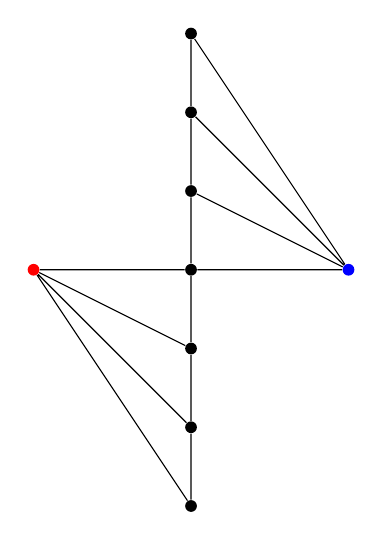
\begin{tikzpicture}[scale=1]
            \node (a) at (2,0) [circle,fill,inner sep=1.5pt] {};
            \node (b) at (2,1) [circle,fill,inner sep=1.5pt] {};
            \node (c) at (2,2) [circle,fill,inner sep=1.5pt] {};
            \node (d) at (2,3) [circle,fill,inner sep=1.5pt] {};
            \node (e) at (2,4) [circle,fill,inner sep=1.5pt] {};
            \node (f) at (2,5) [circle,fill,inner sep=1.5pt] {};
            \node (g) at (2,6) [circle,fill,inner sep=1.5pt] {};

            \node (u) at (0,3) [circle,fill,inner sep=1.5pt, color=red] {};
            \node (v) at (4,3) [circle,fill,inner sep=1.5pt, color=blue] {};
            \draw (u) -- (a) (u) -- (b) (u) -- (c) (u) -- (d) (v) -- (e) (v) -- (f) (v) -- (g)  (v) -- (d)
            (a) -- (b) (b) -- (c) (c) -- (d) (d) -- (e) (e) -- (f) (f) -- (g);

        \end{tikzpicture}
            \caption{\scriptsize Representación de $G$ cuando $|V|$ es impar, suponiendo que en la columna central (negra) son adyacentes cualesquiera 2 vertices.}
       \end{minipage}

        \end{figure}

    \item Para $|V|$ par encuentre una gráfica $\left( \left\lfloor \frac{|V|}{2} \right\rfloor - 1 \right)$-regular e inconexa.\\

        Como podemos ver de dibujar las gráficas para $|V| = 2, |V| = 4, |V| = 6$ y $|V| = 8$\\

    
%Primera fila de graficas
\begin{figure}[h!]
    \centering
    \begin{minipage}{0.2\textwidth}
        \centering
        
\begin{tikzpicture}[scale=1]
            \node (a) at (0,0) [circle,fill,inner sep=1.5pt,color=red] {};
            \node (b) at (0,1) [circle,fill,inner sep=1.5pt] {};

        \end{tikzpicture}
        \caption{\scriptsize Representación de una gráfica $0$-regular de 2 vértices}
    \end{minipage}
    \hspace{0.015\textwidth}
    \begin{minipage}{0.2\textwidth}
        \centering
        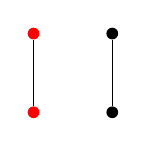
\begin{tikzpicture}[scale=1]
            \node (a) at (0,0) [circle,fill,inner sep=1.5pt,color=red] {};
            \node (b) at (0,1) [circle,fill,inner sep=1.5pt,color=red] {};
            \node (c) at (1,0) [circle,fill,inner sep=1.5pt] {};
            \node (d) at (1,1) [circle,fill,inner sep=1.5pt] {};

            \draw (a) -- (b) (c) -- (d);

        \end{tikzpicture}
        \caption{\scriptsize Representación de una gráfica $1$-regular de 4 vértices}
    \end{minipage}
    \hspace{0.015\textwidth}
    \begin{minipage}{0.2\textwidth}
        \centering
        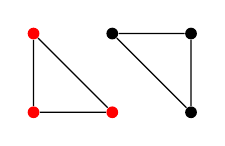
\begin{tikzpicture}[scale=1]
            \node (a) at (0,0) [circle,fill,inner sep=1.5pt,color=red] {};
            \node (b) at (0,1) [circle,fill,inner sep=1.5pt,color=red] {};
            \node (c) at (1,0) [circle,fill,inner sep=1.5pt,color=red] {};
            \node (d) at (1,1) [circle,fill,inner sep=1.5pt] {};
            \node (e) at (2,0) [circle,fill,inner sep=1.5pt] {};
            \node (f) at (2,1) [circle,fill,inner sep=1.5pt] {};


            \draw (a) -- (b) (a) -- (c) (b) -- (c) (d) -- (e) (d) -- (f) (e) -- (f);

        \end{tikzpicture}
        \caption{\scriptsize Representación de una gráfica $2$-regular de 6 vértices}
    \end{minipage}
    \hspace{0.015\textwidth}
    \begin{minipage}{0.2\textwidth}
        \centering
        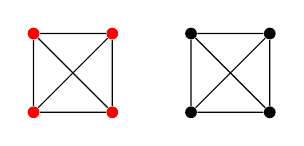
\begin{tikzpicture}[scale=1]
            \node (a) at (0,0) [circle,fill,inner sep=1.5pt,color=red] {};
            \node (b) at (0,1) [circle,fill,inner sep=1.5pt,color=red] {};
            \node (c) at (1,0) [circle,fill,inner sep=1.5pt,color=red] {};
            \node (d) at (1,1) [circle,fill,inner sep=1.5pt,color=red] {};
            \node (e) at (2,0) [circle,fill,inner sep=1.5pt] {};
            \node (f) at (2,1) [circle,fill,inner sep=1.5pt] {};
            \node (g) at (3,0) [circle,fill,inner sep=1.5pt] {};
            \node (h) at (3,1) [circle,fill,inner sep=1.5pt] {};


            \draw (a) -- (b) (a) -- (c) (b) -- (d) (d) -- (c) (a) -- (d) (b) -- (c) (e) -- (f) (f) -- (g) (g) -- (h) (e) -- (g) (f) -- (h) (e) -- (h);

        \end{tikzpicture}
        \caption{\scriptsize Representación de una gráfica $3$-regular de 6 vértices}
    \end{minipage}
\end{figure}

    Podemos decir que las gráficas que representan la condición son las $2k_n$ con $n \geq 1$ y $n \in \mathbb{N}$.

\end{enumerate}

\vspace{1cm}

%
% Ejercicio 5
%
\textbf{5.} Demuestre que si $D$ no tiene lazos y $\delta^+ \geq 1$, entonces $D$ contiene un ciclo dirigido de longitud 
al menos $\delta^+ + 1$.\\

\begin{tcolorbox}[title=\textbf{Hipotesis}, colback=red!15!white, colframe=black!]
    Sabemos que $D$ no tiene lazos y ademas $\delta^{+} \geq 1$.
\end{tcolorbox}
$P.D$ La gráfica $D$ contiene un cilco dirigido de longitud al menos $\delta^{+} + 1$

Sea $D$ una gráfica dirgida que conntiene una trayecttoria dirigida máxima $P$ tal que:
\begin{center}
    $P = (d_1, e_1, d_2, e_2, \dots,d_{k-1}, e_{k - 1}, d_k)$
\end{center}
Como sabemos que P es de longitud máxima y además el exgrado minimo de $D$ es mayor o igual a 1, entonces el vértice $d_k$ tiene 
una arísta saleinte $e_k$ que, por ser $P$ de longitud máxima no puede incidir en un vértice $d_{k +1}$, pues de ser así 
$P$ no sería de lóngitud máxima.\\

De lo anterior, debe haber un vértice $d_i$ en la secuancia de $P$ tal que $d_k$ incide en $d_i = d_{k + 1}$ con $i \in \{1, 2, \dots, k-1\}$,
de no ser así $P$ no sería una trayectoria dirigida de longitud máxima. Con ello deducimos:
\begin{center}
    $P = (d_1, e_1, d_2, e_2,\dots, d_i = d_{k+1}, \dots,d_{k-1}, e_{k - 1}, d_k, e_k, d_i = d_{k+1})$
\end{center}

Como hemos visto que $d_k$ debe incidir en un vértice anterior y perteneciente a $P$ decimos que 
$D$ contiene un ciclo de al menos longitud $\delta^{+} +1$.

\end{document}
